\section{Experimental Results}
This chapter gives an overview of the applied dataset (\cref{sect:staver})
and experimental setup (\cref{sect:exp-setup}). Finally, the results are discussed
in \cref{sect:results-and-discussion}. For the interested reader, an introduction
to the applied metric (\gls{map}) is provided in \cref{sect:metrics}.

\subsection{StaVer}\label{sect:staver}
\Gls{ssd}, as presented in \cref{sect:methodology} will be evaluated on the publicly
available dataset \gls{staver}\footnotemark~\cite{Micenkova.2015}.
\footnotetext{\url{https://madm.dfki.de/downloads-ds-staver}}

From direct examination, the dataset contains 427 images in total. However,
27 images are not annotated and can therefore not be used for train/test splits.
Out of the remaining 400 images, 320 images contain colored and the remaining
80 images contain black stamps.  To reduce computational complexity, a resolution
of 200 dpi is chosen, although 300 and 600 dpi are also available. The dataset
comprises several stamp-categories. Most distinctly, graphical and textual stamps
are included. As an addition to the original dataset, the author has produced
class annotation (``Text'', ``Image'').

For every image, two different \gls{gt} types are available. The former contains
a segmentation map\footnotetext{Meaning that every pixel belonging to a stamp is
marked.}, the latter \gls{gt} \glspl{bbox}. Unfortunately, both given \gls{gt}
types are provided only in form of images \cref{fig:text-stamp-gt,fig:img-stamp-gt}.

Coordinates (as required for \cref{eq:offset-calc}) are extracted from the \gls{gt}
\gls{bbox} images programmatically. OpenCV~\cite{Bradski.2000} is used to find
connected components and convert them into rectangles. Finally, coordinates are
determined using \texttt{cv2.boxPoints(\ldots)}.

\begin{figure}[th!]
    \begin{subfigure}[t]{.225\linewidth}
        \centering
        \includegraphics[width=.9\textwidth]{stampDS-00251.png}
        \subcaption{Textual stamp example from \gls{staver} (stampDS-00251)}\label{fig:text-stamp}
    \end{subfigure}\hfill
    \begin{subfigure}[t]{.225\linewidth}
        \centering
        
\includegraphics[width=.9\textwidth]{stampDS-00251-gt.png}
        \subcaption{Image containing the \gls{gt}\gls{bbox} for the textual stamp (stampDS-00251)}\label{fig:text-stamp-gt}
    \end{subfigure}\hfill
    \begin{subfigure}[t]{.225\linewidth}
        \centering
        \includegraphics[width=.9\textwidth]{stampDS-00138.png}
        \subcaption{Two image-stamps from \gls{staver} (stampDS-00138)}\label{fig:img-stamp}
    \end{subfigure}\hfill
    \begin{subfigure}[t]{.225\linewidth}
        \centering
        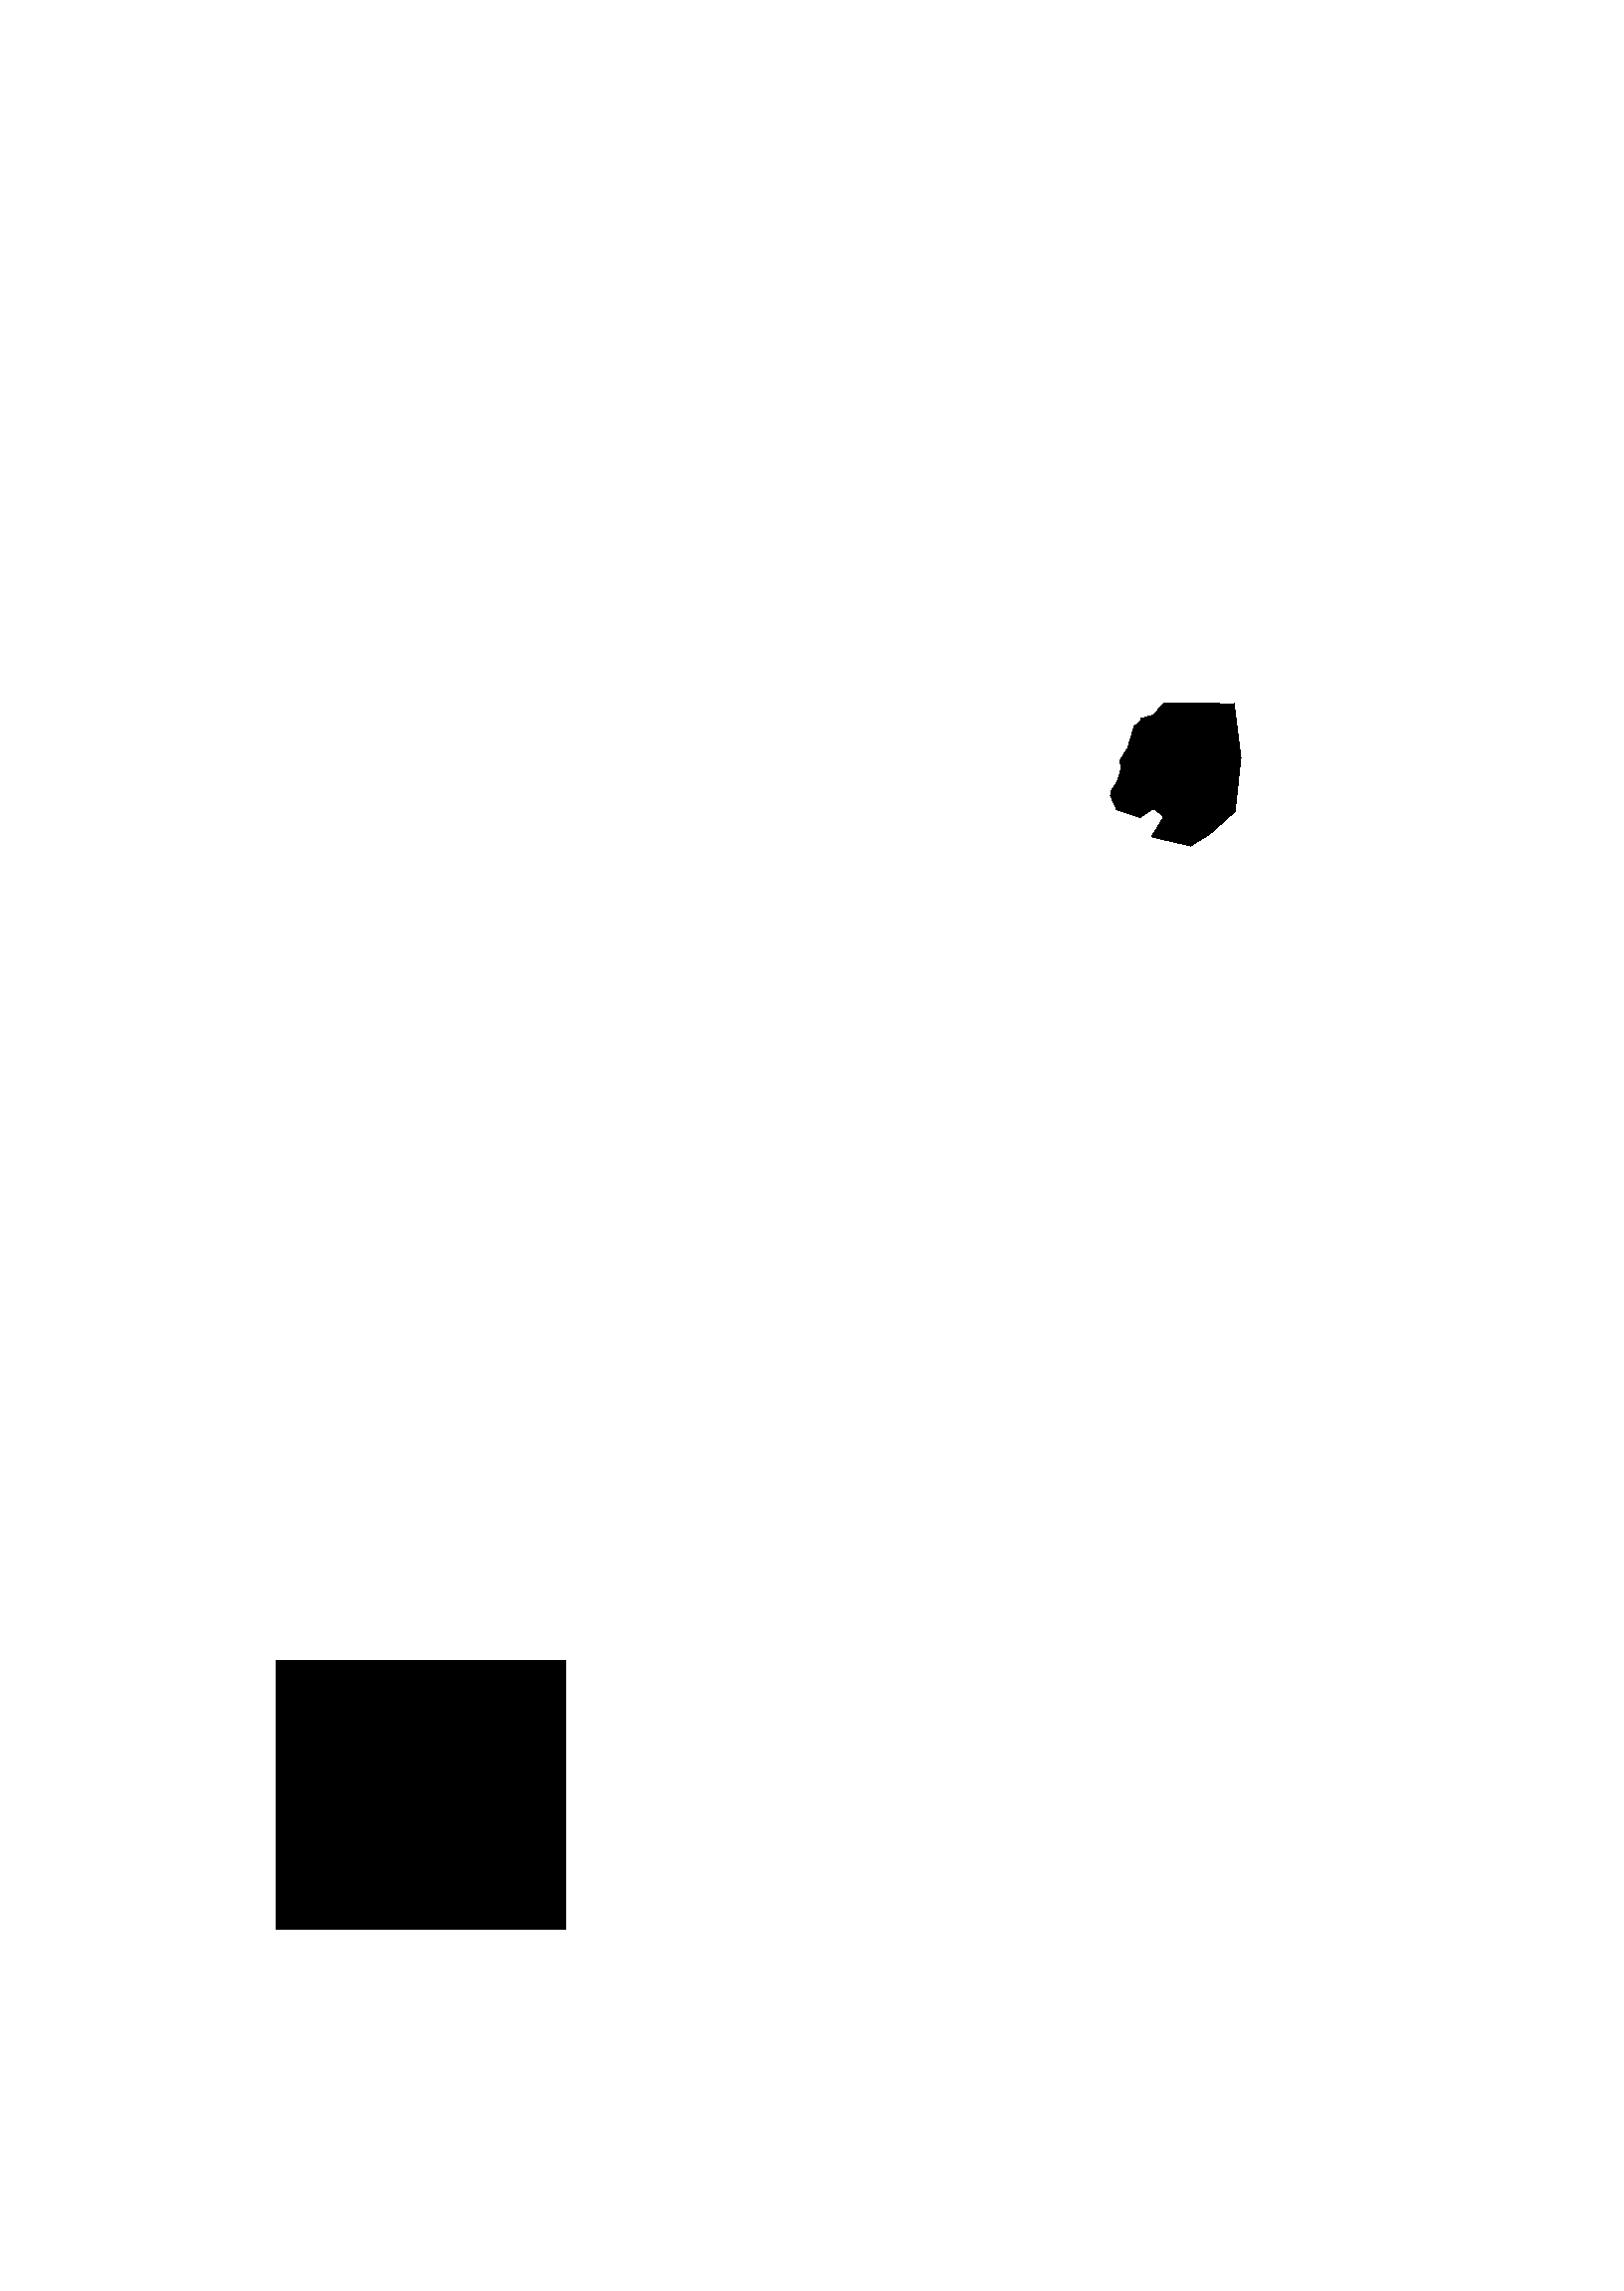
\includegraphics[width=.9\textwidth]{stampDS-00138-gt.png}
        \subcaption{Image containing the \gls{gt}\gls{bbox} for the two image-stamps (stampDS-00138)}\label{fig:img-stamp-gt}
    \end{subfigure}
    \caption[Example images from \gls{staver} and respective \gls{gt}]{Example
    images from \gls{staver} and respective \gls{gt} \glspl{bbox}. Unfortunately,
    \gls{bbox} \gls{gt} is sometimes corrupted, e.g.\ (\subref{fig:img-stamp-gt}).}
\end{figure}

\subsection{Experimental Setup}\label{sect:exp-setup}
For image preprocessing, a set of manipulations
\begin{multline*}
    \{\text{Brightness-jitter, Color-jitter, Saturation-jitter, Horizontal-flip, Vertical-flip, Random-crop,}\\\text{Black-and-White}\}
\end{multline*}
are applied randomly.

\Gls{ssd} is implemented by the author using Python 3.7 and TensorFlow 2.0~\cite{Abadi.2015}.
As base network, MobileNet~\cite[cf.][]{Howard.2017} is adopted without pre-training\footnotemark.
Hyperparameters are chosen as per the original paper, confer~\cite{Liu.2016}.
Training and inference are run using \texttt{NVIDIA DGX A100} infrastructure.

\footnotetext{Common datasets like e.g.\ ImageNet~\cite{Deng.2009} come from a substantially different
distribution. Note please that pre-training and thereby heterogenous transfer learning
\textit{might} be useful nonetheless~\cite{Day.2017}, but would require additional
ablation studies which is beyond the scope of this work.}

Out of the 400 available and annotated images, 65\% (240) are chosen for training
and 35\% (100) are chosen for testing. A validation set is not constructed, because
no hyperparameter optimization is conducted~\cite[cf.][120\psq]{Goodfellow.2016}.

\subsection{Results \& Discussion}\label{sect:results-and-discussion}
Results seem generally competitive with the original implementation by \textcite{Liu.2016}\footnotemark.
Besides that, the results from this work unfortunately cannot be compared to
related approaches in stamp detection which, as noted in \cref{sect:related-work},
were mostly concerned with image segmentation.

As demonstrated in \cref{fig:loss,fig:map-75}, the model converges after about
a 10.000 training steps, reaching its maximum \gls{map}@0.75\gls{iou} of 0.593
after 9.000 training steps.

\footnotetext{Comparing apples and oranges, the best implementation of \gls{ssd}
by \textcite{Liu.2016} reached a \gls{map}@.75\gls{iou} of 30.3[Table 6, \texttt{COCO test-dev2015}]\cite{Liu.2016}.}

\begin{figure}[htp!]
    \centering
    \begin{subfigure}{.49\linewidth}
        \begin{tikzpicture}
            \begin{axis}[cycle list name=tb, 
                        grid=both,
                        grid style={solid,gray!30!white},
                        axis lines=middle,
                        xlabel={step},
                        ylabel={L(l)},
                        x label style={at={(axis description cs:0.5,-0.1)},anchor=north},
                        y label style={at={(axis description cs:-0.1,.5)},rotate=90,anchor=south},]
            \addplot table [x=Step, y=Value, col sep=comma] {loss.csv};
            \end{axis}
        \end{tikzpicture}
        \subcaption{Model loss over time}\label{fig:loss}
    \end{subfigure}
    \hfill
    \begin{subfigure}{.49\linewidth}
        \begin{tikzpicture}
            \begin{axis}[cycle list name=tb, 
                        grid=both,
                        grid style={solid,gray!30!white},
                        axis lines=middle,
                        xlabel={step},
                        ylabel={mAP@75IoU},
                        ytick={0.3,0.4,0.5,0.595},
                        x label style={at={(axis description cs:0.5,-0.1)},anchor=north},
                        y label style={at={(axis description cs:-0.1,.5)},rotate=90,anchor=south},]
            \addplot table [x=Step, y=Value, col sep=comma] {map@75iou.csv};
            \end{axis}
        \end{tikzpicture}
        \subcaption{\gls{map}@.75\gls{iou} computed on the test set}\label{fig:map-75}
    \end{subfigure}
    \caption{Model loss and test metrics over time}
\end{figure}

From visual evaluation, the model is able to overcome most issues noted in
\cref{sect:related-work}. In most cases, black and white stamps could be
identified (see \cref{fig:black-and-white}) as well as stamps with significant
overlap (\cref{fig:diff-domain-overlap,fig:overlap-insample}).

As a downside it is noted that in few cases, \gls{ssd} was vulnerable to
\gls{fp} detections of logos, which look very similar to graphical stamps
(see \cref{fig:logo-as-stamp}). Also, sometimes multiple stamps are detected as
a single stamp (see \cref{fig:multi-as-one}).

Interestingly, also stamps from different distributions could be identified without
significant increase in \glspl{fp} (see \cref{fig-diff-domains}).
